\documentclass[tikz]{standalone}
\usepackage[utf8x]{inputenc}
\usepackage{amsmath}
\usepackage{tikz}
\usetikzlibrary{arrows,matrix,positioning}
\begin{document}
    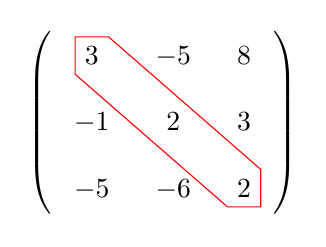
\begin{tikzpicture}
        \matrix [matrix of math nodes,left delimiter=(,right delimiter=), row sep=10pt,column sep = 10pt] (m)
        {
            3 & -5 & 8 \\
            -1 & 2 & 3 \\
            -5 & -6 & 2 \\
        };  
        \draw [color = red] (m-1-1.north west) -- (m-1-1.south west) -- (m-3-3.south west) -- (m-3-3.south east) -- (m-3-3.north east) -- (m-1-1.north east) -- cycle;
    \end{tikzpicture}
\end{document}